% =====================================================================
%  Capítulo 5. Estacionariedad y raíces unitarias
% =====================================================================
\part{Series de tiempo univariadas}

\chapter[Estacionariedad y raíces unitarias]{Estacionariedad, autocorrelación y raíces unitarias}\label{cap:raiz}

\section*{Objetivos de aprendizaje}
Al terminar este capítulo, el lector podrá:
\begin{enumerate}[label=\arabic*.,leftmargin=*]
  \item Definir la estacionariedad y distinguir un proceso estacionario de uno con raíz unitaria por sus
        momentos, sus trayectorias y su función de autocorrelación.
  \item Calcular la persistencia de un proceso autorregresivo con la vida media de un choque.
  \item Explicar por qué una regresión entre series con raíz unitaria puede ser espuria.
  \item Derivar la distribución de Dickey-Fuller y aplicar las pruebas ADF y KPSS con la especificación
        determinista y el número de rezagos adecuados.
  \item Reconocer el efecto de los quiebres estructurales sobre las pruebas de raíz unitaria y aplicar la
        prueba de Zivot-Andrews.
\end{enumerate}

\section*{Motivación}
¿Vuelve el precio del petróleo a un nivel ``normal'' después de una crisis, o cada choque lo deja en un
nivel nuevo, del que parte la siguiente historia? ¿Regresa el miedo del mercado, medido por el VIX, a su
promedio? ¿Fluctúan las tasas de interés de largo plazo alrededor de un valor estable o deambulan sin
ancla? La respuesta a estas preguntas determina casi todo lo que se puede hacer con una serie: si tiene
sentido pronosticarla a largo plazo, si se puede usar en una regresión sin transformar, si sus choques
son transitorios o permanentes.

La herramienta para responderlas es la distinción entre series \emph{estacionarias} y series con
\emph{raíz unitaria}, y las pruebas que permiten decidir entre ambas. Este capítulo abre la Parte~II del
libro: a partir de aquí los datos dejan de ser muestras de observaciones independientes y pasan a ser lo
que realmente son en finanzas: trayectorias en el tiempo.

\paragraph{Datos del capítulo.} Brent diario (1987--2026), VIX diario (1990--2026), tasa de interés del bono
del Tesoro de EE.\,UU. a 10 años y razón dividendo/precio del S\&P 500 (base de Shiller, 1871--2023), y
precio mensual del oro (1975--2026).

% ---------------------------------------------------------------------
\section{Procesos estocásticos y estacionariedad}
% ---------------------------------------------------------------------

Una serie de tiempo $y_1,\dots,y_T$ se interpreta como una realización de un \emph{proceso estocástico}
$\{y_t\}$: una sucesión de variables aleatorias indexadas por el tiempo. Solo observamos una trayectoria;
para aprender algo del proceso a partir de ella, sus propiedades deben ser estables en el tiempo.

\begin{definicion}[Estacionariedad débil]
El proceso $\{y_t\}$ es \emph{débilmente estacionario} (o estacionario en covarianza) si para todo $t$ y todo
$j$:
\begin{align*}
  \E[y_t]            &= \mu,\\
  \Var(y_t)          &= \gamma_0<\infty,\\
  \Cov(y_t,y_{t-j})  &= \gamma_j,
\end{align*}
es decir, la media, la varianza y las autocovarianzas no dependen de $t$, sino solo de la distancia $j$.
La \emph{función de autocorrelación} (ACF) es $\rho_j=\gamma_j/\gamma_0$.
\end{definicion}

\begin{definicion}[Ruido blanco]
Un proceso $\{\varepsilon_t\}$ es \emph{ruido blanco} si tiene media cero, varianza constante $\sigma^2$ y
autocovarianzas nulas: $\gamma_j=0$ para $j\ne0$. Si además las $\varepsilon_t$ son independientes, es ruido
blanco i.i.d. Los rendimientos del Brent del Capítulo~\ref{cap:hechos} son ruido blanco, pero no i.i.d.
\end{definicion}

\begin{definicion}[Autocorrelación parcial]
La \emph{autocorrelación parcial} (PACF) de orden $j$, $\phi_{jj}$, es el último coeficiente de la regresión
poblacional de $y_t$ sobre $y_{t-1},\dots,y_{t-j}$: mide la relación entre $y_t$ y $y_{t-j}$ una vez
descontado el efecto de los rezagos intermedios.
\end{definicion}

\subsection{El proceso autorregresivo de orden 1}

\begin{definicion}[AR(1)]
$y_t=c+\phi\,y_{t-1}+\varepsilon_t$, con $\varepsilon_t$ ruido blanco de varianza $\sigma^2$.
\end{definicion}

\begin{proposicion}[Momentos del AR(1) estacionario]\label{prop:ar1}
Si $|\phi|<1$ y el proceso es estacionario, entonces
\begin{align*}
  \mu      &= \frac{c}{1-\phi},\\
  \gamma_0 &= \frac{\sigma^2}{1-\phi^2},\\
  \rho_j   &= \phi^{\,j}, \qquad j\ge0 .
\end{align*}
\end{proposicion}

\begin{proof}
\emph{Media.} Tomando esperanzas y usando $\E[y_t]=\E[y_{t-1}]=\mu$:
\begin{align*}
  \mu           &= c+\phi\,\mu\\
  \mu-\phi\,\mu &= c\\
  \mu           &= \frac{c}{1-\phi}.
\end{align*}
\emph{Varianza.} Como $\varepsilon_t$ no está correlacionado con $y_{t-1}$, que solo depende de choques
pasados, y $\Var(y_t)=\Var(y_{t-1})=\gamma_0$:
\begin{align*}
  \gamma_0               &= \Var(c+\phi\,y_{t-1}+\varepsilon_t)\\
                         &= \phi^2\,\gamma_0+\sigma^2\\
  \gamma_0\,(1-\phi^2)   &= \sigma^2\\
  \gamma_0               &= \frac{\sigma^2}{1-\phi^2}.
\end{align*}
\emph{Autocovarianzas.} Para $j\ge1$, $\varepsilon_t$ no está correlacionado con $y_{t-j}$:
\begin{align*}
  \gamma_j &= \Cov(y_t,\,y_{t-j})\\
           &= \Cov(c+\phi\,y_{t-1}+\varepsilon_t,\ y_{t-j})\\
           &= \phi\,\Cov(y_{t-1},\,y_{t-j})\\
           &= \phi\,\gamma_{j-1}.
\end{align*}
Aplicando la recursión $j$ veces, $\gamma_j=\phi^{\,j}\gamma_0$, y dividiendo entre $\gamma_0$,
$\rho_j=\phi^{\,j}$.
\end{proof}

La ACF de un AR(1) estacionario decae geométricamente: rápido si $\phi$ es pequeño, lentamente si $\phi$ se
acerca a 1. Su PACF, en cambio, se corta después del primer rezago, porque una vez conocido $y_{t-1}$ los
rezagos anteriores no aportan información sobre $y_t$. La Figura~\ref{fig:procesos} muestra cómo cambia la
trayectoria al aumentar $\phi$.

\begin{proposicion}[Vida media de un choque]\label{prop:vidamedia}
En un AR(1) estacionario con $0<\phi<1$, el efecto de un choque sobre $y_{t+h}$ es $\phi^h$ veces su efecto
inicial. La \emph{vida media}, el número de períodos que tarda en disiparse la mitad del efecto, es
\[
  h^*=\frac{\ln 0{,}5}{\ln\phi}.
\]
\end{proposicion}

\begin{proof}
Sustituyendo hacia atrás $h$ veces la ecuación del AR(1):
\begin{align*}
  y_{t+h} &= c+\phi\,y_{t+h-1}+\varepsilon_{t+h}\\
          &= c\,(1+\phi)+\phi^2\,y_{t+h-2}+\phi\,\varepsilon_{t+h-1}+\varepsilon_{t+h}\\
          &\;\;\vdots\\
          &= c\sum_{i=0}^{h-1}\phi^{\,i}+\phi^{h}\,y_t+\sum_{i=0}^{h-1}\phi^{\,i}\,\varepsilon_{t+h-i}.
\end{align*}
Un choque que eleva $y_t$ en una unidad eleva $y_{t+h}$ en $\phi^h$ unidades. La vida media resuelve
\begin{align*}
  \phi^{h^*}          &= 0{,}5\\
  h^*\,\ln\phi        &= \ln0{,}5\\
  h^*                 &= \frac{\ln0{,}5}{\ln\phi}. && \qedhere
\end{align*}
\end{proof}

\subsection{El paseo aleatorio}

\begin{definicion}[Paseo aleatorio]
Si $\phi=1$ y $c=0$, el AR(1) es un \emph{paseo aleatorio}: $y_t=y_{t-1}+\varepsilon_t$. Si $c\ne0$, es un
paseo aleatorio \emph{con deriva}. Se dice que el proceso tiene una \emph{raíz unitaria}.
\end{definicion}

\begin{proposicion}[Momentos del paseo aleatorio]\label{prop:paseo}
Con $y_0$ fijo, el paseo aleatorio cumple, para $s\le t$:
\begin{align*}
  \E[y_t]                       &= y_0,\\
  \Var(y_t)                     &= t\,\sigma^2,\\
  \Cov(y_t,y_s)                 &= s\,\sigma^2,\\
  \operatorname{Corr}(y_t,y_s)  &= \sqrt{s/t}.
\end{align*}
En particular, no es estacionario: su varianza crece sin límite.
\end{proposicion}

\begin{proof}
Sustituyendo hacia atrás, el paseo es la suma de todos los choques pasados:
\begin{align*}
  y_t &= y_{t-1}+\varepsilon_t\\
      &= y_{t-2}+\varepsilon_{t-1}+\varepsilon_t\\
      &\;\;\vdots\\
      &= y_0+\sum_{i=1}^{t}\varepsilon_i .
\end{align*}
La media es $y_0$ porque cada $\varepsilon_i$ tiene media cero. Como los choques no están correlacionados:
\begin{align*}
  \Var(y_t) &= \sum_{i=1}^{t}\Var(\varepsilon_i)\\
            &= t\,\sigma^2 .
\end{align*}
Para $s\le t$, $y_t$ y $y_s$ comparten los choques $\varepsilon_1,\dots,\varepsilon_s$:
\begin{align*}
  \Cov(y_t,y_s) &= \Cov\Bigl(\sum_{i=1}^{t}\varepsilon_i,\ \sum_{i=1}^{s}\varepsilon_i\Bigr)\\
                &= \sum_{i=1}^{s}\Var(\varepsilon_i)\\
                &= s\,\sigma^2,\\
  \operatorname{Corr}(y_t,y_s) &= \frac{s\,\sigma^2}{\sqrt{t\,\sigma^2}\,\sqrt{s\,\sigma^2}}\\
                               &= \sqrt{\frac{s}{t}}. && \qedhere
\end{align*}
\end{proof}

La última fórmula explica el aspecto de la ACF muestral de un paseo aleatorio: como
$\sqrt{(t-j)/t}\approx1$ cuando $t$ es grande, las autocorrelaciones son cercanas a 1 y decaen muy despacio.
Los choques nunca se disipan: un choque en $t$ desplaza para siempre todo el futuro (su ``vida media'' es
infinita). La Figura~\ref{fig:procesos} compara los cuatro casos.

\begin{figure}[ht]
\centering
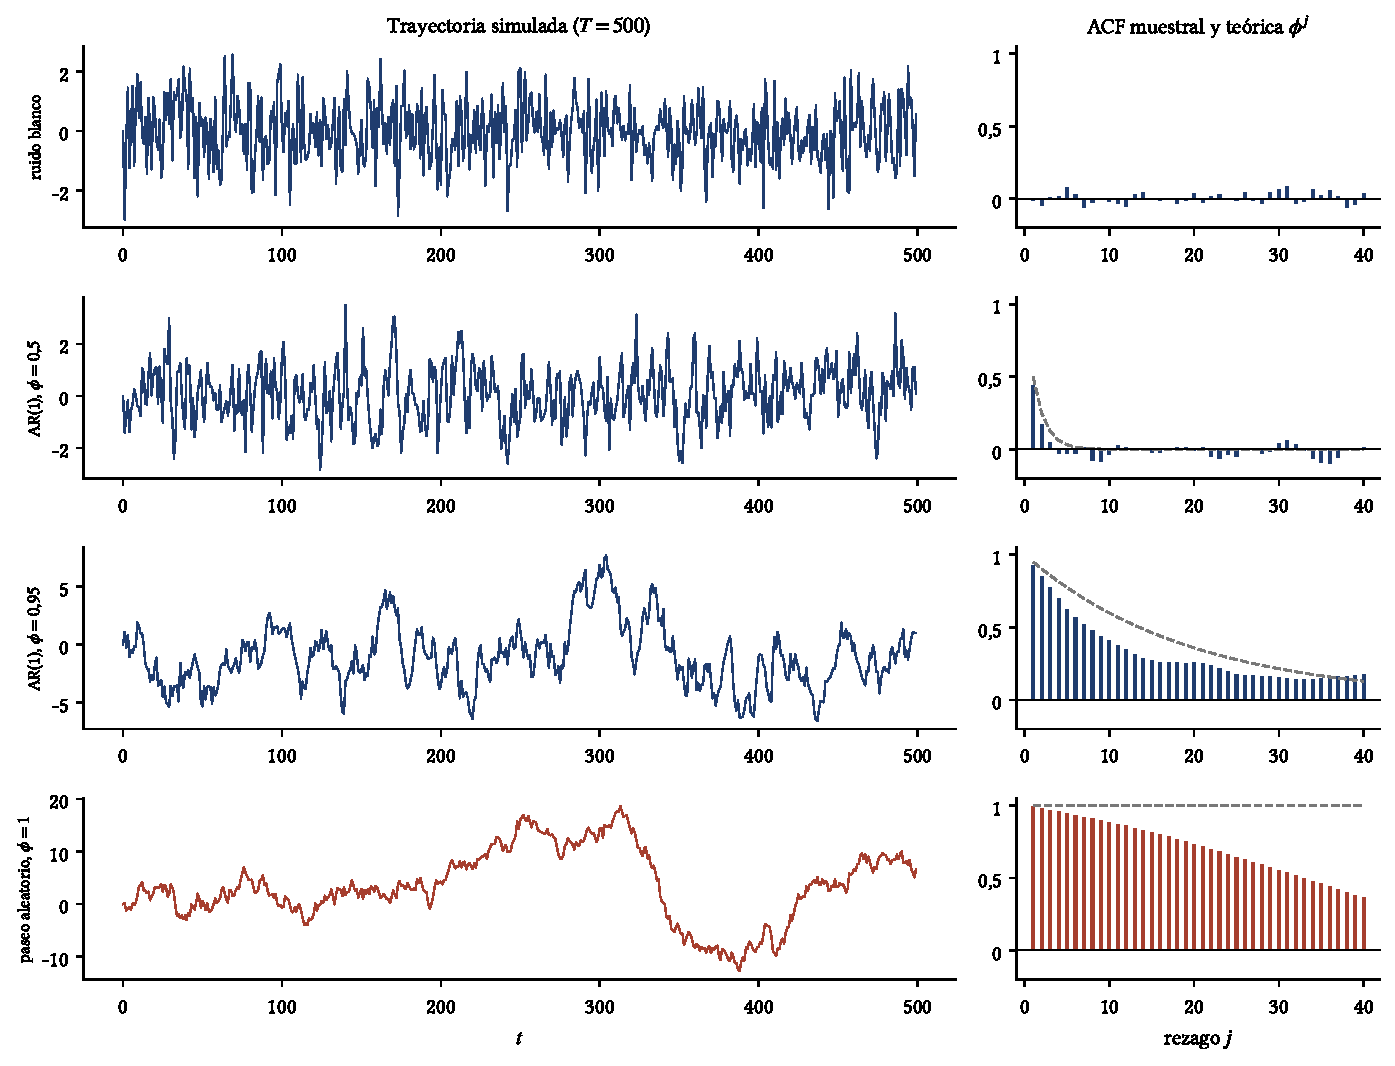
\includegraphics[width=\linewidth]{graficos/cap05_fig_procesos.pdf}
\caption{Trayectorias simuladas con los mismos choques (izquierda) y su ACF muestral (barras) frente a la
teórica $\phi^j$ (línea discontinua). Al aumentar $\phi$, la serie se aleja más tiempo de su media y la ACF
decae más despacio. El paseo aleatorio no tiene media a la que volver: deambula, y su ACF muestral queda
cerca de 1 en todos los rezagos.}
\label{fig:procesos}
\end{figure}

\begin{definicion}[Orden de integración]
Un proceso es \emph{integrado de orden $d$}, $I(d)$, si debe diferenciarse $d$ veces para volverse
estacionario. Un proceso estacionario es $I(0)$; un paseo aleatorio es $I(1)$, porque
$\Delta y_t=y_t-y_{t-1}=\varepsilon_t$ es estacionario. En finanzas, los logaritmos de los precios suelen ser
$I(1)$ y los rendimientos, $I(0)$.
\end{definicion}

\begin{proposicion}[Sobrediferenciación]\label{prop:sobrediferencia}
Si $y_t=\varepsilon_t$ es ruido blanco y se diferencia, $\Delta y_t=\varepsilon_t-\varepsilon_{t-1}$ tiene
autocorrelación de primer orden igual a $-1/2$.
\end{proposicion}

\begin{proof}
\begin{align*}
  \Var(\Delta y_t)                    &= \Var(\varepsilon_t)+\Var(\varepsilon_{t-1})\\
                                      &= 2\sigma^2,\\
  \Cov(\Delta y_t,\Delta y_{t-1})     &= \Cov(\varepsilon_t-\varepsilon_{t-1},\ \varepsilon_{t-1}-\varepsilon_{t-2})\\
                                      &= -\Var(\varepsilon_{t-1})\\
                                      &= -\sigma^2,\\
  \rho_1                              &= \frac{-\sigma^2}{2\sigma^2}\\
                                      &= -\frac12 . && \qedhere
\end{align*}
\end{proof}

Diferenciar una serie que ya era estacionaria no la ``arregla'': introduce una autocorrelación negativa
artificial. Por eso no conviene diferenciar por si acaso; hay que decidir con pruebas formales.

% ---------------------------------------------------------------------
\section{Regresión espuria}
% ---------------------------------------------------------------------

Granger y Newbold (1974) mostraron con simulaciones que, al regresar un paseo aleatorio sobre otro
\emph{independiente}, la prueba $t$ rechaza la hipótesis de pendiente nula con mucha más frecuencia que el
nivel nominal, el $R^2$ suele ser alto y el estadístico de Durbin-Watson, cercano a cero. Phillips (1986)
demostró que el estadístico $t$ no converge a ninguna distribución: crece con $\sqrt T$, de modo que con más
datos el rechazo falso es \emph{más} probable. La intuición es que ambas series tienen tendencias
estocásticas que deambulan, y en cualquier muestra finita esas tendencias parecen relacionadas.

La Figura~\ref{fig:espuria} lo confirma: en 2\,000 simulaciones por tamaño de muestra, la prueba $t$ al 5\,\%
rechaza la hipótesis verdadera de independencia el 66\,\% de las veces con $T=50$ y el 91\,\% con
$T=1\,000$. Si las mismas series se regresan en diferencias, los rechazos vuelven al 5\,\%. Una regla
práctica clásica es sospechar de cualquier regresión en niveles con $R^2$ mayor que el estadístico de
Durbin-Watson.

\begin{figure}[ht]
\centering
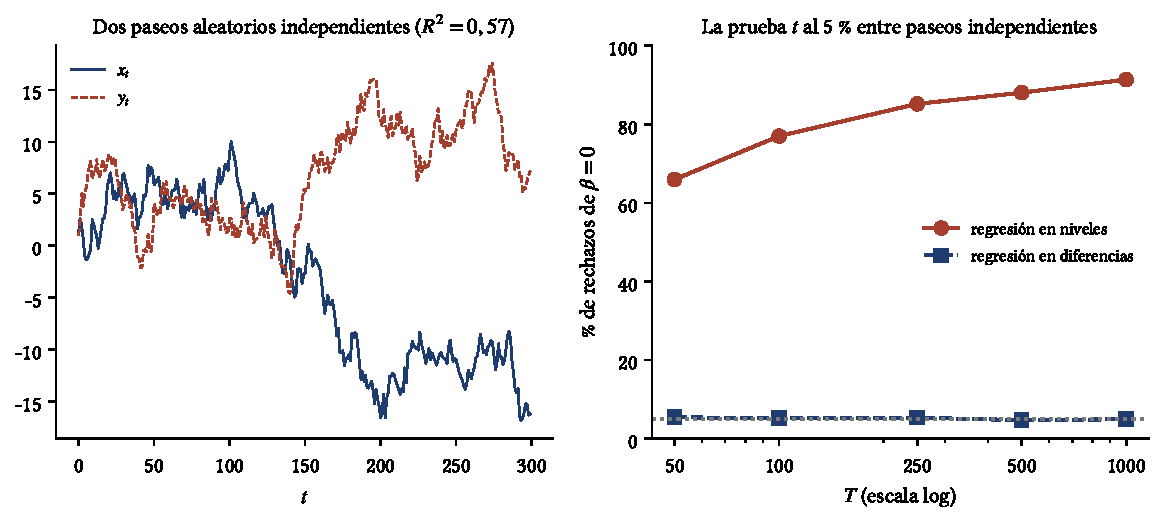
\includegraphics[width=\linewidth]{graficos/cap05_fig_espuria.pdf}
\caption{Izquierda: dos paseos aleatorios independientes, elegidos para ilustrar un caso con $R^2$ alto
($0{,}57$). Derecha: porcentaje de rechazos de $H_0:\beta=0$, que es cierta, con la prueba $t$ al 5\,\%.
En niveles, el rechazo falso aumenta con el tamaño de la muestra; en diferencias, se mantiene en el 5\,\%.}
\label{fig:espuria}
\end{figure}

% ---------------------------------------------------------------------
\section{La prueba de Dickey-Fuller}
% ---------------------------------------------------------------------

Para decidir si una serie tiene raíz unitaria, la idea natural es estimar
$y_t=\phi y_{t-1}+\varepsilon_t$ y probar $H_0:\phi=1$. Restando $y_{t-1}$ en ambos lados, la regresión
equivalente es
\[
  \Delta y_t=\gamma\,y_{t-1}+\varepsilon_t,\qquad \gamma=\phi-1,
\]
y la hipótesis nula es $H_0:\gamma=0$ (raíz unitaria) frente a $H_1:\gamma<0$ (estacionariedad). El problema
es que, bajo la hipótesis nula, el estimador no tiene la distribución habitual.

\begin{teorema}[Dickey-Fuller]\label{teo:df}
Si $y_t=y_{t-1}+\varepsilon_t$ con $y_0=0$ y $\varepsilon_t$ i.i.d. con varianza $\sigma^2$, el estimador MCO
$\hat\phi$ de la regresión sin constante cumple
\[
  T(\hat\phi-1)\ \xrightarrow{d}\ \frac{\tfrac12\bigl[W(1)^2-1\bigr]}{\int_0^1W(r)^2\,dr},
\]
donde $W$ es un movimiento browniano estándar. En particular, $\hat\phi$ converge a 1 a la velocidad $T$ (no
$\sqrt T$), y la distribución límite no es normal.
\end{teorema}

\begin{proof}
El estimador MCO es $\hat\phi=\sum_ty_{t-1}y_t/\sum_ty_{t-1}^2$. Como $y_t=y_{t-1}+\varepsilon_t$:
\begin{align*}
  \hat\phi-1 &= \frac{\sum_ty_{t-1}(y_{t-1}+\varepsilon_t)}{\sum_ty_{t-1}^2}-1\\
             &= \frac{\sum_ty_{t-1}\,\varepsilon_t}{\sum_ty_{t-1}^2}.
\end{align*}
Multiplicamos el numerador y el denominador por potencias de $T$ que los estabilizan:
\[
  T(\hat\phi-1)=\frac{T^{-1}\sum_ty_{t-1}\varepsilon_t}{T^{-2}\sum_ty_{t-1}^2}.
\]
\emph{Numerador.} Elevando al cuadrado la ecuación del paseo:
\begin{align*}
  y_t^2                    &= (y_{t-1}+\varepsilon_t)^2\\
                           &= y_{t-1}^2+2\,y_{t-1}\varepsilon_t+\varepsilon_t^2\\
  y_{t-1}\,\varepsilon_t   &= \tfrac12\bigl(y_t^2-y_{t-1}^2-\varepsilon_t^2\bigr).
\end{align*}
Sumando de $t=1$ a $T$, la suma de $y_t^2-y_{t-1}^2$ es telescópica y $y_0=0$:
\begin{align*}
  \sum_{t=1}^Ty_{t-1}\,\varepsilon_t &= \tfrac12\Bigl(y_T^2-y_0^2-\sum_{t=1}^T\varepsilon_t^2\Bigr)\\
                                     &= \tfrac12\Bigl(y_T^2-\sum_{t=1}^T\varepsilon_t^2\Bigr),\\
  \frac1{T\sigma^2}\sum_{t=1}^Ty_{t-1}\,\varepsilon_t
                                     &= \frac12\Bigl[\Bigl(\frac{y_T}{\sigma\sqrt T}\Bigr)^2-\frac{1}{T\sigma^2}\sum_{t=1}^T\varepsilon_t^2\Bigr].
\end{align*}
Por el teorema central del límite, $y_T/(\sigma\sqrt T)\to W(1)\sim N(0,1)$, y por la ley de los grandes
números, $\frac1{T\sigma^2}\sum_t\varepsilon_t^2\to1$. El numerador converge a
$\tfrac12\bigl[W(1)^2-1\bigr]$.

\emph{Denominador.} El teorema central del límite funcional (principio de invariancia de Donsker) establece
que la trayectoria reescalada $y_{\lfloor rT\rfloor}/(\sigma\sqrt T)$, $r\in[0,1]$, converge a $W(r)$. Como
$\frac{1}{T^2\sigma^2}\sum_ty_{t-1}^2$ es una suma de Riemann de $\bigl(y_{\lfloor rT\rfloor}/(\sigma\sqrt T)\bigr)^2$,
converge a $\int_0^1W(r)^2dr$. Aplicando el teorema de la aplicación continua al cociente se obtiene el
resultado (los $\sigma^2$ se cancelan).
\end{proof}

Dos consecuencias se leen directamente de la fórmula. Primera, como $W(1)^2\sim\chi^2_1$, el numerador es
negativo cuando $W(1)^2<1$, lo que ocurre con probabilidad $P(|Z|<1)=0{,}683$: $\hat\phi$ tiende a quedar
\emph{por debajo} de 1 y la distribución está sesgada a la izquierda. Segunda, el estadístico $t$ de
$\hat\gamma$ tampoco es normal; también converge a un funcional del browniano, que depende de los términos
deterministas incluidos en la regresión.

\paragraph{Términos deterministas.} En la práctica se estima una de tres regresiones: sin términos
deterministas, con constante ($\Delta y_t=\alpha+\gamma y_{t-1}+\varepsilon_t$, adecuada para series sin
tendencia, como tasas de interés o razones financieras), o con constante y tendencia lineal (adecuada para
series con tendencia, como el logaritmo de un índice bursátil). Cada caso tiene su propia distribución bajo
$H_0$. La Figura~\ref{fig:df} muestra las tres, obtenidas por simulación, y la Tabla~\ref{tab:vcdf} compara
los cuantiles simulados con los valores asintóticos de MacKinnon (2010).

\begin{figure}[ht]
\centering
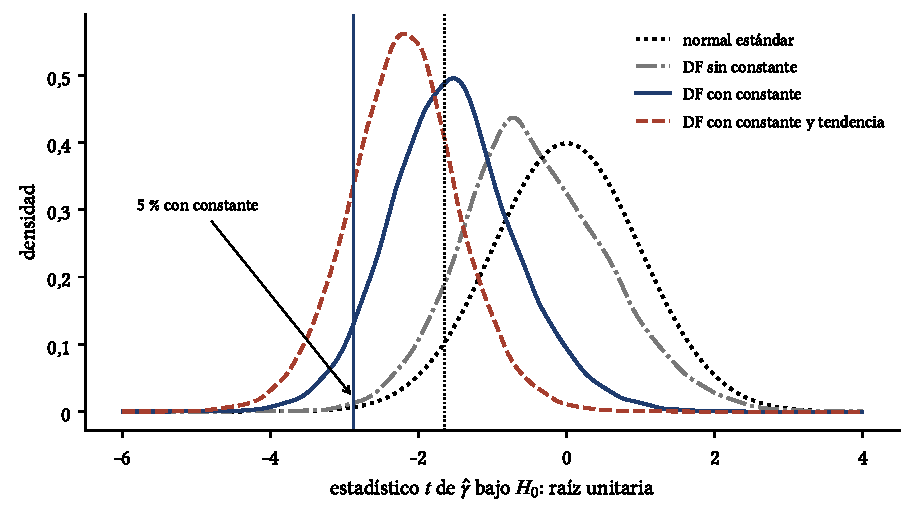
\includegraphics[width=0.82\linewidth]{graficos/cap05_fig_df.pdf}
\caption{Distribución del estadístico $t$ de Dickey-Fuller bajo la hipótesis de raíz unitaria (20\,000
simulaciones con $T=500$), frente a la normal estándar. Las tres distribuciones están desplazadas a la
izquierda, y más cuantos más términos deterministas incluye la regresión. Usar el valor crítico normal
($-1{,}645$, línea punteada) llevaría a rechazar la raíz unitaria con demasiada frecuencia.}
\label{fig:df}
\end{figure}

\begin{table}[ht]
\centering\small
\begin{tabular}{@{}lccccccc@{}}
\toprule
 & \multicolumn{3}{c}{Simulación ($T=500$)} & & \multicolumn{3}{c}{MacKinnon (asintóticos)} \\
\cmidrule{2-4}\cmidrule{6-8}
Regresión & 1\,\% & 5\,\% & 10\,\% & & 1\,\% & 5\,\% & 10\,\% \\
\midrule
Sin constante              & $-2{,}52$ & $-1{,}94$ & $-1{,}62$ & & $-2{,}57$ & $-1{,}94$ & $-1{,}62$ \\
Con constante              & $-3{,}46$ & $-2{,}88$ & $-2{,}59$ & & $-3{,}43$ & $-2{,}86$ & $-2{,}57$ \\
Con constante y tendencia  & $-3{,}97$ & $-3{,}42$ & $-3{,}14$ & & $-3{,}96$ & $-3{,}41$ & $-3{,}13$ \\
\bottomrule
\end{tabular}
\caption{Valores críticos del estadístico $t$ de Dickey-Fuller. Las simulaciones están en
\texttt{cap05\_figuras\_teoria.py}; las pequeñas diferencias con los valores asintóticos se deben al tamaño
finito de la muestra y al error de simulación.}
\label{tab:vcdf}
\end{table}

\subsection{Dickey-Fuller aumentada (ADF)}

Si los errores de la regresión están autocorrelacionados, la distribución anterior deja de valer. La
solución de Said y Dickey (1984) es añadir rezagos de la variable dependiente:
\[
  \Delta y_t=\alpha+\beta t+\gamma\,y_{t-1}+\sum_{j=1}^{p}\delta_j\,\Delta y_{t-j}+\varepsilon_t,
\]
con los términos deterministas que correspondan. El estadístico es el $t$ de $\hat\gamma$ y se compara con
los mismos valores críticos. El número de rezagos $p$ se elige con un criterio de información (en este libro,
el AIC) en una muestra común, partiendo de un máximo $p_{\max}=\lfloor12(T/100)^{1/4}\rfloor$ (Schwert, 1989).

\subsection{Phillips-Perron}

Phillips y Perron (1988) proponen otra solución: estimar la regresión de Dickey-Fuller sin rezagos y
corregir el estadístico $t$ con una estimación no paramétrica de la varianza de largo plazo, del mismo tipo
que el estimador de Newey-West del Capítulo~\ref{cap:robustos}. Tiene la misma distribución límite que la
prueba ADF y es robusta a heterocedasticidad de forma general, pero en muestras finitas suele tener peor
tamaño cuando los errores tienen autocorrelación negativa fuerte.

% ---------------------------------------------------------------------
\section{La prueba KPSS: estacionariedad como hipótesis nula}
% ---------------------------------------------------------------------

Las pruebas ADF y PP tienen poca potencia frente a alternativas muy persistentes: con $\phi=0{,}98$ es muy
difícil distinguir un AR(1) de un paseo aleatorio en una muestra moderada. Como la hipótesis nula es la
raíz unitaria, ``no rechazar'' es la respuesta por defecto cuando los datos no son concluyentes. Kwiatkowski,
Phillips, Schmidt y Shin (1992) invierten las hipótesis.

\begin{definicion}[Prueba KPSS]
Sea $\hat e_t$ el residuo de regresar $y_t$ sobre una constante (o sobre una constante y una tendencia), y
$S_t=\sum_{s=1}^t\hat e_s$ su suma parcial. El estadístico es
\[
  \eta=\frac{1}{T^2\,\hat\sigma^2_{\mathrm{LP}}}\sum_{t=1}^TS_t^2,
\]
donde $\hat\sigma^2_{\mathrm{LP}}$ es la varianza de largo plazo de $\hat e_t$, estimada con el núcleo de
Bartlett y $l$ rezagos. La hipótesis nula es la estacionariedad y se rechaza para valores \emph{grandes} de
$\eta$. Los valores críticos al 10\,\%, 5\,\% y 1\,\% son $0{,}347$; $0{,}463$ y $0{,}739$ con constante, y
$0{,}119$; $0{,}146$ y $0{,}216$ con tendencia.
\end{definicion}

La intuición está en la Figura~\ref{fig:kpss}. Si la serie es estacionaria, sus desviaciones respecto de la
media se compensan y las sumas parciales oscilan cerca de cero. Si tiene raíz unitaria, pasa largos períodos
por encima o por debajo de su media muestral, y las sumas parciales se alejan mucho: $\eta$ es grande.

\begin{figure}[ht]
\centering
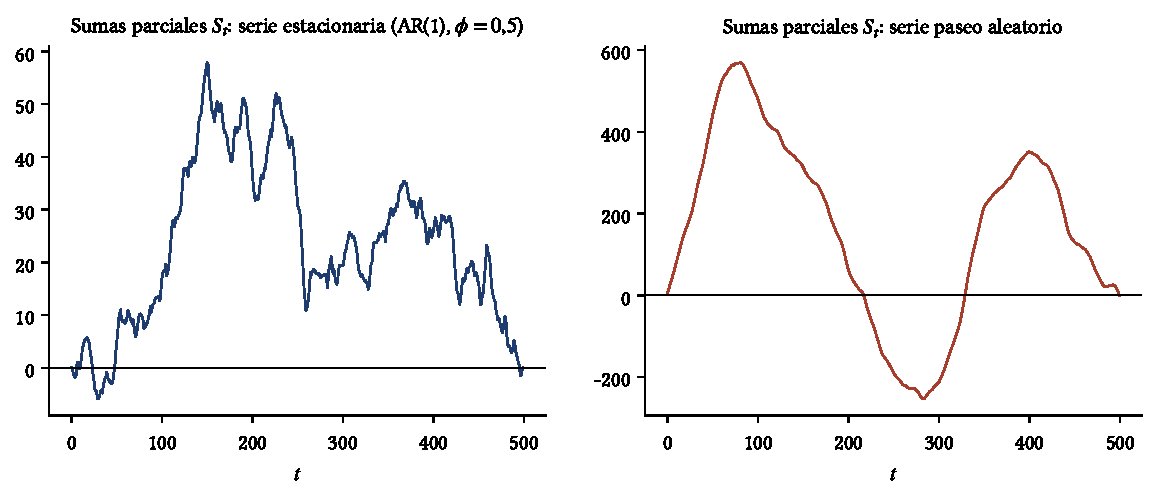
\includegraphics[width=\linewidth]{graficos/cap05_fig_kpss.pdf}
\caption{Sumas parciales de las desviaciones respecto de la media para una serie estacionaria (izquierda) y
para un paseo aleatorio (derecha). Observe la escala: en el paseo aleatorio son decenas de veces mayores.}
\label{fig:kpss}
\end{figure}

\paragraph{Análisis confirmatorio.} Usar juntas las pruebas ADF y KPSS da cuatro resultados posibles:
\begin{center}\small
\begin{tabular}{@{}lll@{}}
\toprule
ADF (nula: raíz unitaria) & KPSS (nula: estacionaria) & Conclusión \\
\midrule
Rechaza       & No rechaza & Estacionaria \\
No rechaza    & Rechaza    & Raíz unitaria \\
No rechaza    & No rechaza & Datos poco informativos \\
Rechaza       & Rechaza    & Ni una cosa ni la otra: memoria larga o quiebres \\
\bottomrule
\end{tabular}
\end{center}

% ---------------------------------------------------------------------
\section{Quiebres estructurales y raíces unitarias}
% ---------------------------------------------------------------------

Perron (1989) mostró que una serie estacionaria con un cambio de nivel puede parecer un paseo aleatorio: el
salto es un choque ``permanente'', y la prueba ADF lo interpreta como evidencia de raíz unitaria. La
Figura~\ref{fig:perron} muestra un ejemplo: un AR(1) con $\phi=0{,}9$ y un salto de 10 unidades a mitad de la
muestra. En 2\,000 simulaciones, la prueba ADF rechaza la raíz unitaria solo el 0,1\,\% de las veces; si se
elimina el salto, la rechaza el 99,8\,\%.

\begin{figure}[ht]
\centering
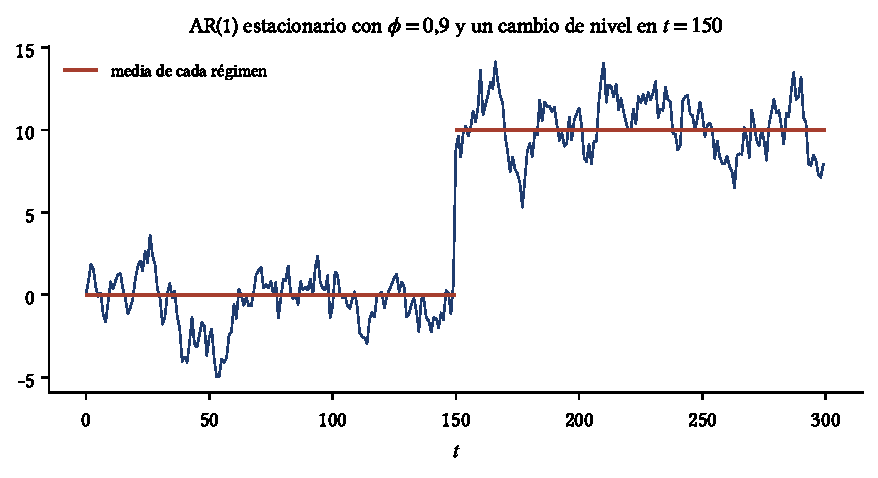
\includegraphics[width=0.82\linewidth]{graficos/cap05_fig_perron.pdf}
\caption{Una serie estacionaria alrededor de una media que cambia una sola vez. Dentro de cada régimen la
serie vuelve rápidamente a su media; vista en conjunto, parece haberse desplazado para siempre, como un
paseo aleatorio.}
\label{fig:perron}
\end{figure}

\begin{definicion}[Prueba de Zivot-Andrews]
Para cada fecha candidata $T_B$ entre el 15\,\% y el 85\,\% de la muestra se estima
\[
  \Delta y_t=\alpha+\theta\,DU_t(T_B)+\beta t+\gamma\,y_{t-1}+\sum_{j=1}^p\delta_j\,\Delta y_{t-j}+\varepsilon_t,
  \qquad DU_t(T_B)=\mathbb 1\{t\ge T_B\},
\]
y se toma el mínimo de los estadísticos $t$ de $\hat\gamma$. La hipótesis nula es la raíz unitaria sin
quiebre; la alternativa, estacionariedad con un cambio de nivel en una fecha desconocida. Los valores
críticos son más negativos que los de ADF: $-5{,}34$, $-4{,}80$ y $-4{,}58$ al 1\,\%, 5\,\% y 10\,\%
(Zivot y Andrews, 1992).
\end{definicion}

% ---------------------------------------------------------------------
\section{Ejercicios resueltos}
% ---------------------------------------------------------------------

Las pruebas ADF y KPSS están programadas desde las fórmulas del texto en los archivos
\texttt{cap05\_funciones} de las carpetas de código de R y de Python, que se muestran en el primer
ejercicio. En Python comprobamos cada resultado con el paquete \texttt{arch}.

\begin{ejresuelto}{¿Tiene raíz unitaria el precio del petróleo?}\label{ej:brentur}
\enunciado Con el Brent diario: (a) aplique las pruebas ADF y KPSS al logaritmo del precio, con constante y
con constante y tendencia; (b) aplíquelas al rendimiento logarítmico; (c) concluya el orden de integración.

\solucion
\paso{Paso 1. Logaritmo del precio.} El AIC elige $p=29$ rezagos. Con constante:
\begin{align*}
  t_{\mathrm{ADF}} &= -1{,}912\\
                   &> -2{,}86 \quad\text{(valor crítico al 5\,\%)},\\
  \eta_{\mathrm{KPSS}} &= 16{,}749\\
                       &> 0{,}463 \quad\text{(valor crítico al 5\,\%)}.
\end{align*}
La prueba ADF no rechaza la raíz unitaria y la KPSS rechaza la estacionariedad con mucha holgura. Con
tendencia, $t_{\mathrm{ADF}}=-3{,}179>-3{,}41$ y $\eta=2{,}622>0{,}146$: la conclusión no cambia.

\paso{Paso 2. Rendimiento.} Con $p=28$ rezagos:
\begin{align*}
  t_{\mathrm{ADF}}     &= -17{,}108 < -2{,}86,\\
  \eta_{\mathrm{KPSS}} &= 0{,}027 < 0{,}463 .
\end{align*}
ADF rechaza la raíz unitaria y KPSS no rechaza la estacionariedad.

\paso{Paso 3. Conclusión.} El logaritmo del precio del Brent es $I(1)$ y su rendimiento es $I(0)$. Los
choques al precio del petróleo son permanentes: la caída de 2020 no fue ``revertida'' por una fuerza que
devolviera el precio a un nivel normal; el precio partió desde su nuevo nivel.

\codigoweb{cap05_ej01}
\salidaR{cap05_ej01_R.txt}
\lectura{cap05_ej01}

\RvsPy Las funciones están escritas de forma paralela en los dos lenguajes, y la única diferencia de fondo
es la indexación: en R la primera fila de la regresión es \texttt{p + 1} y en Python \texttt{p}. La salida
de Python incluye la comprobación con \texttt{arch}: con el mismo número de rezagos, los estadísticos
coinciden en todas las cifras, y \texttt{arch} añade los $p$-valores de MacKinnon. En R el paquete
\texttt{urca} ofrece las mismas pruebas.

\begin{figure}[ht]
\centering
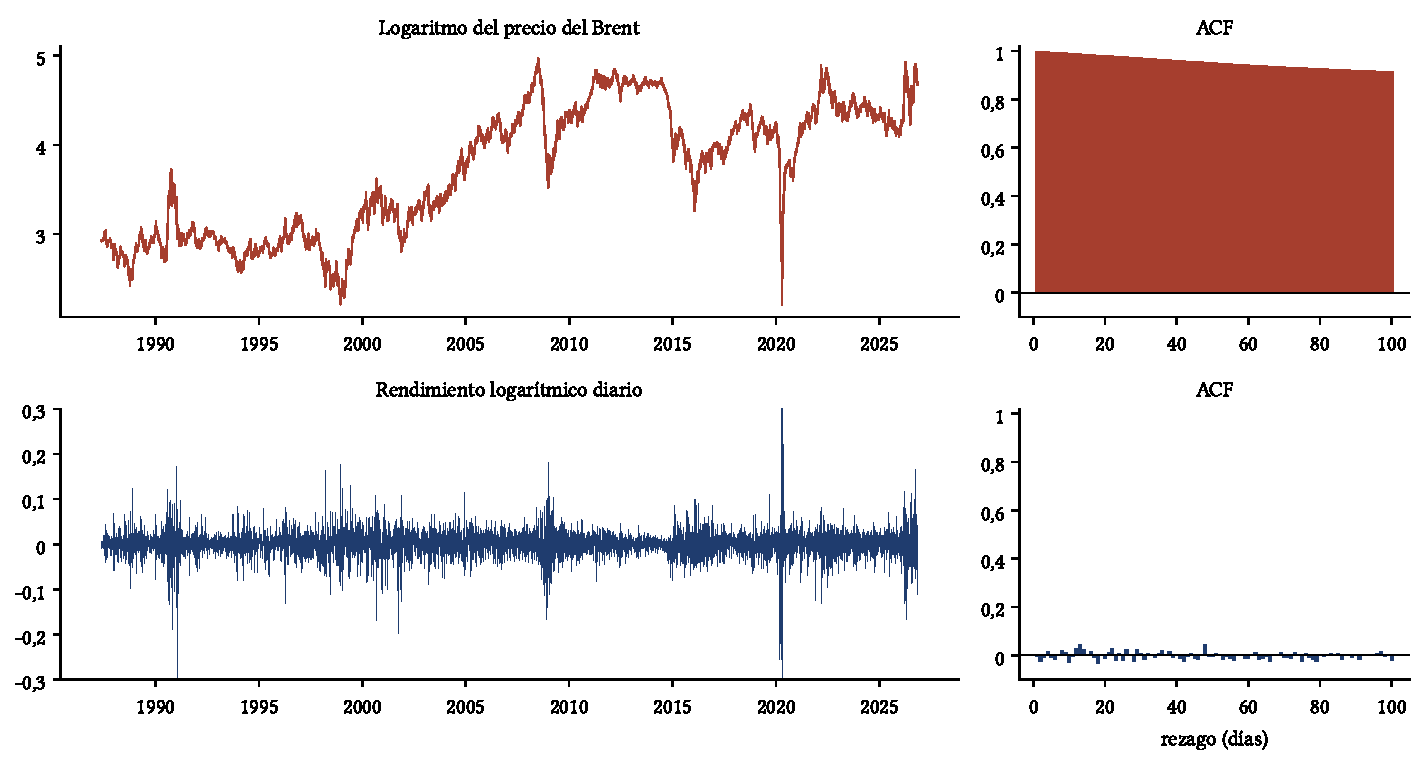
\includegraphics[width=\linewidth]{graficos/cap05_fig_brent.pdf}
\caption{Arriba: el logaritmo del precio del Brent deambula sin una media a la que volver, y su ACF casi no
decae. Abajo: el rendimiento oscila alrededor de cero, con la ACF de un ruido blanco.}
\label{fig:brentur}
\end{figure}

\begin{conclusion}
El precio del petróleo tiene raíz unitaria y su rendimiento es estacionario, como predice la hipótesis de
mercados eficientes. Los modelos de los capítulos siguientes se estiman sobre rendimientos.
\end{conclusion}
\end{ejresuelto}

\begin{ejresuelto}{El VIX: estacionario, pero persistente}\label{ej:vixur}
\enunciado Con el logaritmo del VIX diario: (a) aplique las pruebas ADF y KPSS con constante; (b) estime un
AR(1) y calcule su media de largo plazo y la vida media de un choque; (c) interprete el conjunto de
resultados.

\solucion
\paso{Paso 1. Pruebas.}
\begin{align*}
  t_{\mathrm{ADF}}     &= -6{,}539 < -2{,}86,\\
  \eta_{\mathrm{KPSS}} &= 0{,}568 > 0{,}463 .
\end{align*}
ADF rechaza con claridad la raíz unitaria. KPSS rechaza la estacionariedad al 5\,\%, aunque no al 1\,\%
(valor crítico $0{,}739$). Es el cuarto caso del análisis confirmatorio: ambas rechazan.

\paso{Paso 2. AR(1).} La estimación MCO da $\hat c=0{,}05824$ y $\hat\phi=0{,}97994$. Entonces
\begin{align*}
  \hat\mu &= \frac{\hat c}{1-\hat\phi}\\
          &= \frac{0{,}05824}{1-0{,}97994}\\
          &= 2{,}903,\\
  e^{\hat\mu} &= 18{,}23 .
\end{align*}
El VIX tiende a volver a un nivel de 18,2 puntos. La vida media de un choque es
\begin{align*}
  h^* &= \frac{\ln0{,}5}{\ln\hat\phi}\\
      &= \frac{-0{,}69315}{\ln0{,}97994}\\
      &= \frac{-0{,}69315}{-0{,}02026}\\
      &= 34{,}2 \text{ días}.
\end{align*}

\paso{Paso 3. Interpretación.} El VIX vuelve a su media: un salto del miedo del mercado se reduce a la mitad
en unas siete semanas de negociación. La Figura~\ref{fig:vixur} muestra, sin embargo, que la ACF decae mucho
más despacio que $\hat\phi^j$: a 250 días es $0{,}35$, cuando el AR(1) predice $0{,}006$. Esa es la huella de la \emph{memoria
larga}, un comportamiento intermedio entre $I(0)$ e $I(1)$ que explica por qué las dos pruebas rechazan a la
vez: la serie es demasiado persistente para KPSS y demasiado reversible para ADF.

\codigoweb{cap05_ej02}
\salidaR{cap05_ej02_R.txt}
\lectura{cap05_ej02}

\RvsPy En R, \texttt{lm(y[-1] \textasciitilde{} y[-T])} regresa cada valor sobre el anterior quitando el
primero y el último elemento; en Python se obtiene lo mismo con \texttt{y[1:]} y \texttt{y[:-1]}.

\begin{figure}[ht]
\centering
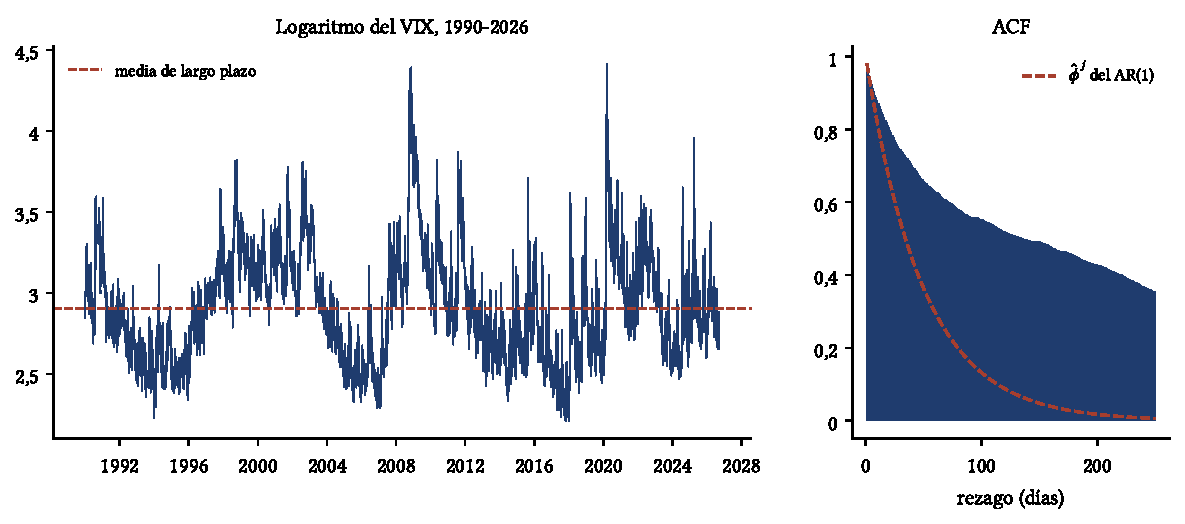
\includegraphics[width=\linewidth]{graficos/cap05_fig_vix.pdf}
\caption{Izquierda: el logaritmo del VIX vuelve siempre a su media de largo plazo, aunque con episodios largos
lejos de ella (2008, 2020). Derecha: su ACF decae mucho más despacio que la de un AR(1) con el mismo
$\hat\phi$.}
\label{fig:vixur}
\end{figure}

\begin{conclusion}
El VIX es estacionario en el sentido económico relevante: vuelve a su media, con una vida media de unos 34
días hábiles. Pero su dependencia de largo plazo es más fuerte que la de un AR(1), un rasgo que comparten
la volatilidad y el volumen de casi todos los activos (Capítulo~\ref{cap:hechos}).
\end{conclusion}
\end{ejresuelto}

\begin{ejresuelto}{La tasa de interés de largo plazo: la prueba ADF paso a paso}\label{ej:tasaur}
\enunciado Con el rendimiento mensual del bono del Tesoro de EE.\,UU. a 10 años (1871--2023): (a) elija el
número de rezagos por AIC; (b) estime la regresión ADF con constante y calcule el estadístico; (c) repita en
diferencias y con la prueba KPSS.

\solucion
\paso{Paso 1. Rezagos.} Con $T=1\,830$ meses, el máximo es
\begin{align*}
  p_{\max} &= \Bigl\lfloor 12\Bigl(\frac{1\,830}{100}\Bigr)^{1/4}\Bigr\rfloor\\
           &= \lfloor 12\times2{,}068\rfloor\\
           &= \lfloor 24{,}8\rfloor\\
           &= 24,
\end{align*}
y el AIC elige $p=22$.

\paso{Paso 2. Estadístico.} En la regresión ADF, $\hat\gamma=-0{,}00288$ con error estándar $0{,}00169$:
\begin{align*}
  t_{\mathrm{ADF}} &= \frac{\hat\gamma}{\operatorname{ee}(\hat\gamma)}\\
                   &= \frac{-0{,}00288}{0{,}00169}\\
                   &= -1{,}70,
\end{align*}
($-1{,}701$ con todos los decimales), mayor que $-2{,}57$, el valor crítico al 10\,\%: no se rechaza la raíz
unitaria. El coeficiente implica $\hat\phi=1+\hat\gamma=0{,}99712$, una persistencia altísima.

\paso{Paso 3. Diferencias y KPSS.} En diferencias, $t_{\mathrm{ADF}}=-10{,}373$: se rechaza la raíz unitaria.
KPSS da $\eta=1{,}164$ en niveles (rechaza la estacionariedad) y $\eta=0{,}075$ en diferencias (no la
rechaza). La tasa de interés se comporta como $I(1)$.

\paso{Paso 4. Interpretación.} Una tasa de interés no puede ser un paseo aleatorio en sentido estricto:
estaría acotada por debajo y la economía no permite que crezca sin límite. Lo que dice la prueba es que su
reversión a la media, si existe, es tan lenta que en 150 años de datos no se distingue de una raíz unitaria.
A efectos prácticos de modelación (Capítulos~10 y~11) se trata como $I(1)$.

\codigoweb{cap05_ej03}
\salidaR{cap05_ej03_R.txt}
\lectura{cap05_ej03}

\RvsPy Al leer el CSV, R convierte el nombre de columna \texttt{Long Interest Rate} en
\texttt{Long.Interest.Rate} (reemplaza los espacios por puntos); \texttt{pandas} conserva el nombre original.

\begin{figure}[ht]
\centering
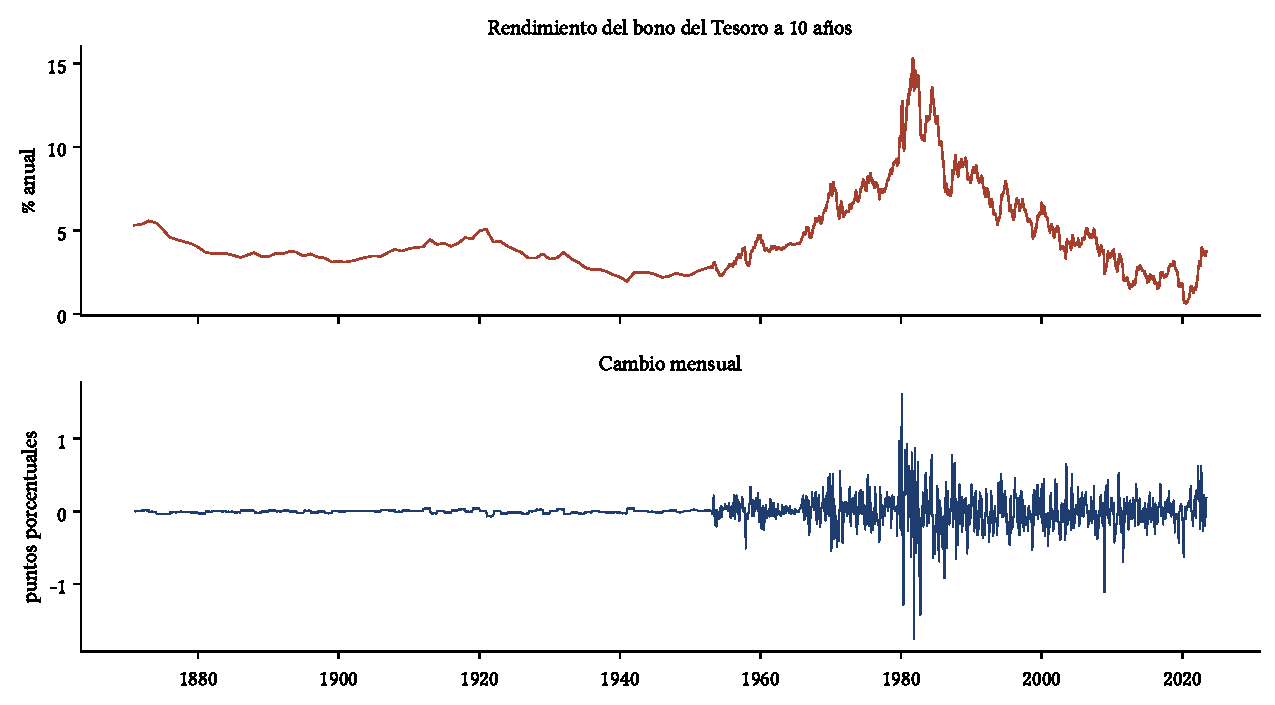
\includegraphics[width=0.9\linewidth]{graficos/cap05_fig_tasa.pdf}
\caption{Arriba: la tasa a 10 años pasa décadas lejos de cualquier promedio (el mínimo de los años cuarenta,
el máximo de 1981, los mínimos de 2020). Abajo: sus cambios mensuales oscilan alrededor de cero, con
volatilidad mucho mayor a partir de los años setenta.}
\label{fig:tasaur}
\end{figure}

\begin{conclusion}
La tasa de interés de largo plazo es $I(1)$ para fines estadísticos. Esto tiene consecuencias inmediatas:
una regresión de otra variable en niveles sobre la tasa de interés corre el riesgo de ser espuria, salvo que
exista cointegración (Capítulo~11).
\end{conclusion}
\end{ejresuelto}

\begin{ejresuelto}{Oro y acciones: una regresión espuria con datos reales}\label{ej:oroespuria}
\enunciado Con datos mensuales de 1975 a 2026: (a) verifique que los logaritmos del precio del oro y del
S\&P 500 son $I(1)$; (b) regrese el primero sobre el segundo en niveles y reporte $\hat b$, $t$, $R^2$ y el
estadístico de Durbin-Watson; (c) haga la misma regresión en diferencias; (d) interprete.

\solucion
\paso{Paso 1. Orden de integración.} En niveles, $t_{\mathrm{ADF}}=-0{,}861$ (oro) y $-0{,}091$ (S\&P 500),
lejos de $-2{,}86$; en diferencias, $-7{,}391$ y $-9{,}919$. Las dos series son $I(1)$.

\paso{Paso 2. Niveles.} Con $T=621$ meses:
\begin{align*}
  \hat b &= 0{,}530, & t &= 32{,}85, & R^2 &= 0{,}636, & DW &= 0{,}0096 .
\end{align*}
Según esta regresión, un aumento de 1\,\% en el S\&P 500 se asocia con un aumento de 0,53\,\% en el oro, con
un estadístico $t$ enorme. Pero la regla de Granger y Newbold se cumple con creces:
\begin{align*}
  R^2 = 0{,}636 &> DW = 0{,}0096 .
\end{align*}
Además, el ADF de los residuos es $-2{,}100$. Con los valores críticos de Dickey-Fuller ($-1{,}94$ sin
constante) parecería rechazar la raíz unitaria, pero esos valores no son válidos para residuos estimados: MCO
elige la recta que hace los residuos lo más estacionarios posible. Los valores críticos correctos (de
Engle-Granger, Capítulo~11) son de alrededor de $-3{,}34$ al 5\,\% para dos variables, y $-2{,}100$ no los
alcanza: no hay evidencia de que las series compartan una tendencia común.

\paso{Paso 3. Diferencias.}
\begin{align*}
  \hat b &= 0{,}015, & t &= 0{,}30, & R^2 &= 0{,}00015 .
\end{align*}
Los rendimientos mensuales del oro y del S\&P 500 no están relacionados.

\codigoweb{cap05_ej04}
\salidaR{cap05_ej04_R.txt}
\lectura{cap05_ej04}

\RvsPy Unimos las dos bases por mes con \texttt{merge} en R y \texttt{merge} en \texttt{pandas}. La base de
Shiller tiene fechas completas (\texttt{1975-01-01}) y la del oro solo año y mes (\texttt{1975-01}), así que
primero extraemos los siete primeros caracteres. Si se unieran por la fecha completa, la intersección
quedaría vacía sin ningún mensaje de error.

\begin{figure}[ht]
\centering
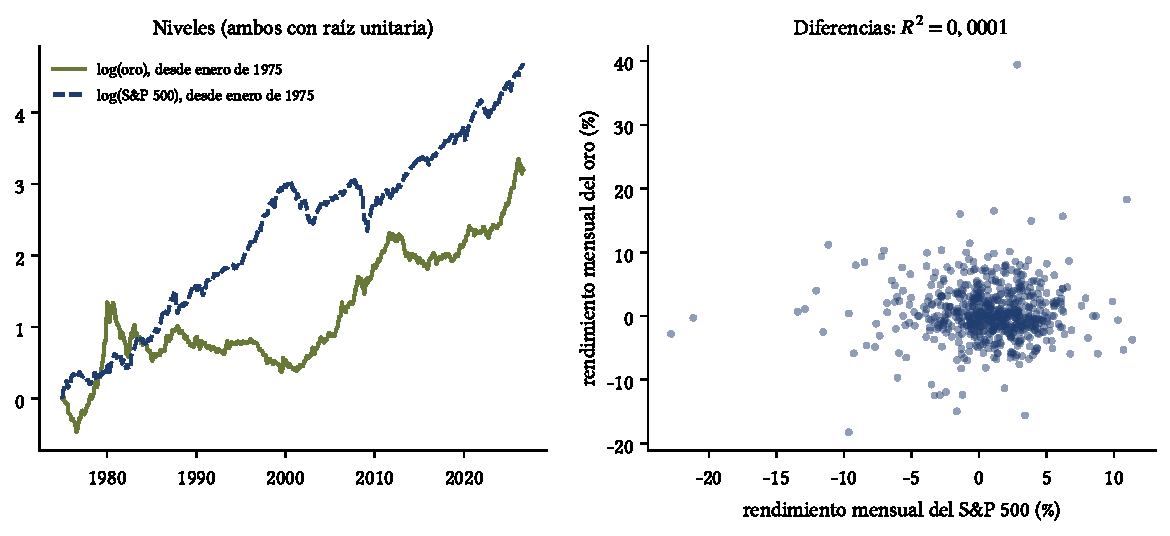
\includegraphics[width=\linewidth]{graficos/cap05_fig_oro.pdf}
\caption{Izquierda: los dos precios crecieron en el largo plazo, y eso basta para que una regresión en niveles
encuentre una relación ``muy significativa''. Derecha: los rendimientos mensuales no muestran ninguna
relación.}
\label{fig:oro}
\end{figure}

\begin{conclusion}
La relación en niveles entre el oro y las acciones es espuria: refleja que ambas series tienen tendencias
estocásticas, no que una explique a la otra. Antes de interpretar una regresión entre series financieras en
niveles hay que verificar su orden de integración y, si son $I(1)$, si están cointegradas.
\end{conclusion}
\end{ejresuelto}

\begin{ejresuelto}{¿Raíz unitaria o quiebre? La razón dividendo/precio}\label{ej:zaur}
\enunciado Con el logaritmo de la razón dividendo/precio del S\&P 500 (1871--2023): (a) aplique la prueba ADF
con tendencia; (b) aplique la prueba de Zivot-Andrews con cambio de nivel, programada a mano, y compárela con
el paquete \texttt{arch}; (c) interprete la fecha del quiebre.

\solucion
\paso{Paso 1. ADF.} Con $p=21$ rezagos, $t_{\mathrm{ADF}}=-2{,}915>-3{,}41$: no se rechaza la raíz unitaria.
Esto es incómodo para la teoría: si la razón dividendo/precio tuviera raíz unitaria, precios y dividendos se
alejarían sin límite, y la regresión predictiva del Ejercicio~\ref{ej:dprediccion} sería espuria.

\paso{Paso 2. Zivot-Andrews.} Recorriendo las 1\,282 fechas candidatas entre el 15\,\% y el 85\,\% de la
muestra, el mínimo del estadístico es
\begin{align*}
  t_{\mathrm{ZA}} &= -4{,}354 \quad\text{(noviembre de 1990)}\\
                  &> -4{,}80 \quad\text{(valor crítico al 5\,\%)}.
\end{align*}
El paquete \texttt{arch} da el mismo valor, con $p=0{,}169$. Ni siquiera permitiendo un cambio de nivel se
rechaza la raíz unitaria.

\paso{Paso 3. Interpretación.} La fecha elegida coincide con un hecho documentado: desde los años noventa las
empresas estadounidenses sustituyeron dividendos por recompras de acciones, y la razón dividendo/precio cayó
a un nivel permanentemente más bajo (Lettau y Van Nieuwerburgh, 2008). Pero el estadístico no alcanza el
valor crítico: con un solo quiebre de nivel, la serie sigue pareciendo $I(1)$. Puede deberse a que hay más de
un quiebre, a que la reversión es muy lenta o a la baja potencia de las pruebas. En el Capítulo~17 volveremos
a esta serie con modelos de cambio de régimen.

\codigoweb{cap05_ej05}
\salidaR{cap05_ej05_R.txt}
\lectura{cap05_ej05}

\RvsPy Lo más delicado es definir la variable indicadora: la fila $k$ de la regresión explica $\Delta y$ en el
período $k+1$, así que $DU=1$ cuando $k+1\ge T_B$. Con esa convención, las versiones de R (índices desde 1) y
de Python (desde 0) recorren las mismas fechas y coinciden con \texttt{arch}.

\begin{figure}[ht]
\centering
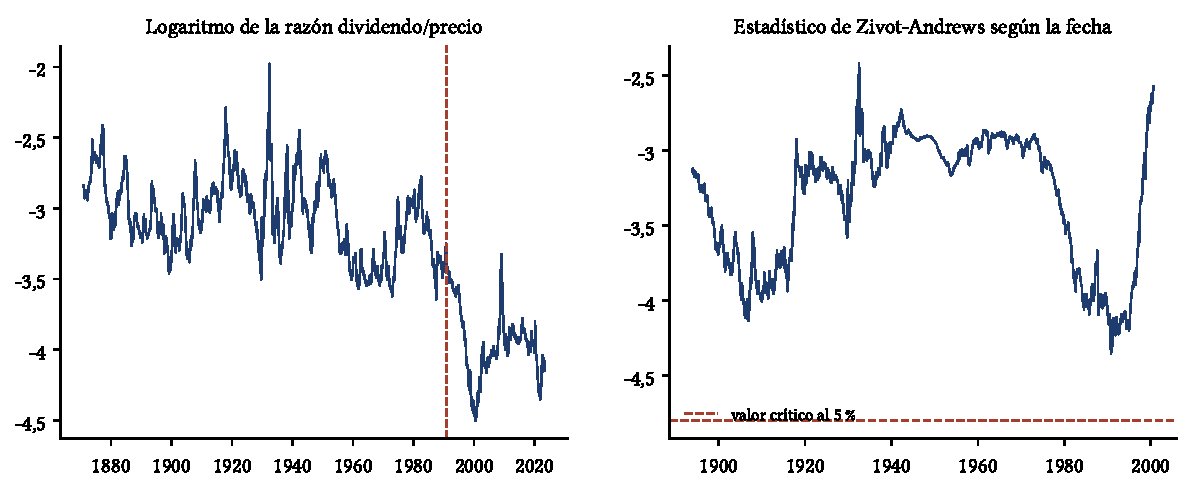
\includegraphics[width=\linewidth]{graficos/cap05_fig_za.pdf}
\caption{Izquierda: la razón dividendo/precio, con la fecha de quiebre que elige la prueba (noviembre de
1990). Derecha: el estadístico de Zivot-Andrews para cada fecha candidata; nunca baja del valor crítico al
5\,\%.}
\label{fig:za}
\end{figure}

\begin{conclusion}
La razón dividendo/precio es extremadamente persistente, con un probable cambio de nivel en los años noventa,
pero las pruebas no permiten rechazar que tenga raíz unitaria. Este es un ejemplo de lo difícil que es, con
datos financieros, separar raíces unitarias, quiebres y reversión lenta.
\end{conclusion}
\end{ejresuelto}

% ---------------------------------------------------------------------
\section{Ejercicios propuestos}
% ---------------------------------------------------------------------

\begin{enumerate}[label=\textbf{\thechapter.\arabic*},leftmargin=*,itemsep=6pt]
  \item Demuestre que en un AR(1) estacionario la PACF es $\phi_{11}=\phi$ y $\phi_{jj}=0$ para $j\ge2$.
  \textit{Pista: escriba la regresión poblacional de $y_t$ sobre $y_{t-1}$ y $y_{t-2}$ y use la
  Proposición~\ref{prop:ar1}.}

  \item Calcule la vida media de un choque si $\phi=0{,}5$; $0{,}9$; $0{,}99$ y $0{,}999$, con datos diarios.
  \textit{Respuesta: 1,0; 6,6; 69,0 y 692,8 días.}

  \item Para un paseo aleatorio con deriva, $y_t=c+y_{t-1}+\varepsilon_t$, demuestre que
  $\E[y_t]=y_0+c\,t$. ¿Por qué la prueba ADF con solo constante es inadecuada para esta serie?

  \item Demuestre que $P\bigl(T(\hat\phi-1)<0\bigr)\to P(\chi^2_1<1)=0{,}683$ bajo la hipótesis de raíz
  unitaria, usando el Teorema~\ref{teo:df}. ¿Qué implica para el sesgo de $\hat\phi$?

  \item \emph{(Simulación.)} Modifique \texttt{cap05\_figuras\_teoria.py} para estimar la potencia de la
  prueba ADF con constante (proporción de rechazos) cuando la serie es un AR(1) con $\phi=0{,}95$, para
  $T=100$, $250$ y $1\,000$. ¿Cuántos años de datos mensuales se necesitan para distinguir $\phi=0{,}95$ de
  una raíz unitaria con una potencia del 80\,\%?

  \item \emph{(Con datos.)} Aplique las pruebas ADF y KPSS al logaritmo del S\&P 500 de Shiller, con constante
  y tendencia. ¿Es $I(1)$? ¿Qué pasa con la inflación mensual calculada a partir del IPC de la misma base?

  \item \emph{(Con datos del BCRP.)} Aplique las pruebas ADF, KPSS y Zivot-Andrews al tipo de cambio
  interbancario soles por dólar desde 2000. ¿Detecta la prueba de Zivot-Andrews un quiebre? ¿En qué fecha?

  \item \emph{(Con datos del BCRP.)} Aplique las pruebas a la tasa de referencia de la política monetaria del
  BCRP. Discuta por qué una serie que el banco central fija por decisión administrativa puede comportarse
  estadísticamente como $I(1)$.
\end{enumerate}

% ---------------------------------------------------------------------
\section{Resumen de fórmulas}
% ---------------------------------------------------------------------

\begin{table}[H]
\centering\small
\begin{tabular}{@{}ll@{}}
\toprule
Concepto & Fórmula \\
\midrule
AR(1) estacionario & $\mu=c/(1-\phi)$;\quad $\gamma_0=\sigma^2/(1-\phi^2)$;\quad $\rho_j=\phi^j$ \\
Vida media & $h^*=\ln0{,}5/\ln\phi$ \\
Paseo aleatorio & $\Var(y_t)=t\sigma^2$;\quad $\operatorname{Corr}(y_t,y_s)=\sqrt{s/t}$ \\
Sobrediferenciación & $\rho_1(\Delta\varepsilon_t)=-1/2$ \\
Dickey-Fuller & $T(\hat\phi-1)\to\frac12[W(1)^2-1]/\int_0^1W^2$ \\
ADF & $\Delta y_t=\alpha+\beta t+\gamma y_{t-1}+\sum_{j=1}^p\delta_j\Delta y_{t-j}+\varepsilon_t$ \\
Valores críticos ADF al 5\,\% & $-1{,}94$ (sin constante);\quad $-2{,}86$ (constante);\quad $-3{,}41$ (tendencia) \\
KPSS & $\eta=\sum_tS_t^2/(T^2\hat\sigma^2_{\mathrm{LP}})$;\quad 5\,\%: $0{,}463$ (constante), $0{,}146$ (tendencia) \\
Zivot-Andrews (cambio de nivel) & 5\,\%: $-4{,}80$ \\
\bottomrule
\end{tabular}
\caption{Fórmulas principales del Capítulo 5.}
\end{table}

\section*{Referencias}
\begin{itemize}[leftmargin=*]
  \item Dickey, D. A. y Fuller, W. A. (1979). Distribution of the estimators for autoregressive time series
        with a unit root. \emph{Journal of the American Statistical Association}, 74(366), 427--431.
  \item Granger, C. W. J. y Newbold, P. (1974). Spurious regressions in econometrics. \emph{Journal of
        Econometrics}, 2(2), 111--120.
  \item Hamilton, J. D. (1994). \emph{Time Series Analysis}. Princeton University Press. Capítulos 3 y 17.
  \item Kwiatkowski, D., Phillips, P. C. B., Schmidt, P. y Shin, Y. (1992). Testing the null hypothesis of
        stationarity against the alternative of a unit root. \emph{Journal of Econometrics}, 54(1--3),
        159--178.
  \item Lettau, M. y Van Nieuwerburgh, S. (2008). Reconciling the return predictability evidence.
        \emph{The Review of Financial Studies}, 21(4), 1607--1652.
  \item MacKinnon, J. G. (2010). Critical values for cointegration tests. Queen's Economics Department
        Working Paper No. 1227.
  \item Perron, P. (1989). The great crash, the oil price shock, and the unit root hypothesis.
        \emph{Econometrica}, 57(6), 1361--1401.
  \item Phillips, P. C. B. (1986). Understanding spurious regressions in econometrics. \emph{Journal of
        Econometrics}, 33(3), 311--340.
  \item Phillips, P. C. B. y Perron, P. (1988). Testing for a unit root in time series regression.
        \emph{Biometrika}, 75(2), 335--346.
  \item Said, S. E. y Dickey, D. A. (1984). Testing for unit roots in autoregressive-moving average models of
        unknown order. \emph{Biometrika}, 71(3), 599--607.
  \item Schwert, G. W. (1989). Tests for unit roots: a Monte Carlo investigation. \emph{Journal of Business
        \& Economic Statistics}, 7(2), 147--159.
  \item Zivot, E. y Andrews, D. W. K. (1992). Further evidence on the great crash, the oil-price shock, and the
        unit-root hypothesis. \emph{Journal of Business \& Economic Statistics}, 10(3), 251--270.
\end{itemize}
